 \section{INTRODU{\c C}{\~A}O}

O Departamento de Computa{\c c}{\~a}o da Faculdade de Ci{\^e}ncias
da UNESP, campus de Bauru, participa de competi{\c c}ões de
futebol de rob{\^o}s, na modalidade Very Small Size (atualmente
IEEE Very Small), desde 1998, com a realiza{\c c}{\~a}o do 1\textordmasculine
Campeonato Brasileiro de Futebol de Rob{\^o}s -- CBFR 98. A
pesquisa e o desenvolvimento em futebol de rob{\^o}s, atualmente
pelo Grupo de Integra{\c c}{\~a}o de Sistemas e Dispositivos
Inteligentes (GISDI), mant{\'e}m o objetivo de incentivar o uso de
inova{\c c}ões tecnol{\'o}gicas, no campo da rob{\'o}tica, de baixo custo e
com componentes encontrados no mercado nacional. Apesar
de diversos per{\'i}odos de aus{\^e}ncia, o time de futebol da UNESP
de Bauru {\'e} conhecido, desde a primeira edi{\c c}{\~a}o desta
competi{\c c}{\~a}o no Brasil, como Carrossel Caipira devido sua
estrat{\'e}gia de jogo. O projeto atual {\'e} a quinta vers{\~a}o, de rob{\^o}s
desenvolvidos para futebol de rob{\^o}s, com aprimoramentos em
rela{\c c}{\~a}o ao time de 2015.

No ambiente do futebol de rob{\^o}s, nesta categoria, os rob{\^o}s
e a bola s{\~a}o identificados atrav{\'e}s de uma c{\^a}mera utilizada
como vis{\~a}o global, posicionada a 2m sobre o campo e alinhada
ao seu centro, que captura imagens da arena. Estas imagens s{\~a}o
processadas digitalmente obtendo as coordenadas dos rob{\^o}s da bola.
A partir dessas coordenadas, uma estrat{\'e}giaescolhida e transformada em comandos que s{\~a}o enviados aos
rob{\^o}s por r{\'a}dio. Os rob{\^o}s recebem estes comandos e realizam
as a{\c c}ões correspondentes, modificando a posi{\c c}{\~a}o dos
elementos presentes no ambiente real, que ser{\'a} capturado
novamente pela c{\^a}mera. A Fig. 1 apresenta uma ilustra{\c c}{\~a}o do
ambiente do futebol de rob{\^o}s.

% FIGURA 1
\begin{figure}[!htb]
\centering
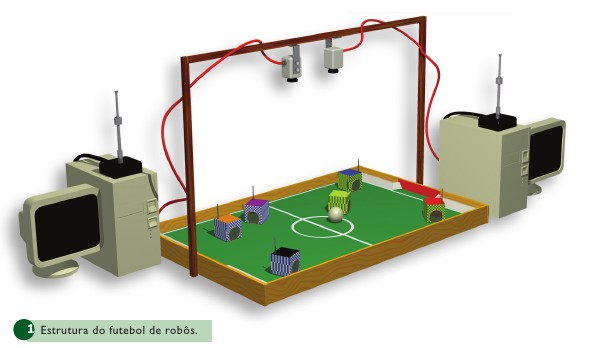
\includegraphics[scale=0.5]{fut_robos.png}
\caption{Ambiente para futebol de rob{\^o}s. Fonte:www.mecatronicaatual.com.br/secoes/leitura/950 (2013)}
\label{Rotulo}
\end{figure}
%%%

O futebol rob{\'o}tico abrange diversas {\'a}reas do conhecimento.
Na constru{\c c}{\~a}o do rob{\^o} s{\~a}o aplicados conceitos de mec{\^a}nica,
eletr{\^o}nica e sistemas embarcados. Do ponto de vista do
software, executado no computador pessoal, est{\~a}o envolvidos
elementos de processamento de imagens, intelig{\^e}ncia artificial
e teoria de controle. Essa abrang{\^e}ncia faz desta modalidade de
futebol uma ferramenta pedag{\'o}gica com poss{\'i}veis aplica{\c c}ões
no ensino.
Esse projeto busca incentivar e facilitar o desenvolvimento
da rob{\'o}tica, para isso o artigo faz uma apresenta{\c c}{\~a}o das tarefas
realizadas, enfatizando a melhoria aplicada recentemente no
simulador do ambiente para divulgar a efici{\^e}ncia obtida ap{\'o}s
essa modifica{\c c}{\~a}o.